% NOTE -- ONLY EDIT Rgraphviz.Rnw!!!
% Rgraphviz.tex file will get overwritten.
%
%\VignetteIndexEntry{A New Interface to Plot Graphs Using Rgraphviz}
%\VignetteDepends{Rgraphviz, graph}
%\VignetteKeywords{tools, graphs}
%\VignettePackage{Rgraphviz}

\documentclass{article}
\usepackage{hyperref}

\newcommand{\Rfunction}[1]{{\texttt{#1}}}
\newcommand{\Rpackage}[1]{{\textit{#1}}}
\newcommand{\Robject}[1]{{\texttt{#1}}}
\newcommand{\Rclass}[1]{{\textit{#1}}}
\newcommand{\R}[0]{{\textit{R}}}

\newcommand{\inclfig}[3]{%
 \begin{figure}[htbp] \begin{center}
   \includegraphics[width=#2]{#1}
   \caption{\label{#1}#3}
 \end{center} \end{figure}
}

\author{Florian Hahne}
\usepackage{Sweave}
\begin{document}
\Sconcordance{concordance:newRgraphvizInterface.tex:newRgraphvizInterface.Rnw:%
1 25 1 1 0 69 1 1 2 1 0 6 1 4 0 1 2 40 1 1 2 1 0 1 1 4 0 1 2 45 1 1 2 1 %
0 1 1 4 0 1 2 35 1 1 2 1 0 1 1 4 0 1 2 3 1 1 2 1 0 3 1 4 0 1 2 1 1 1 2 %
1 0 1 1 4 0 1 2 25 1 1 4 3 0 1 1 4 0 1 2 32 1 1 2 1 0 1 1 4 0 1 2 13 1 %
1 3 2 0 1 1 4 0 1 2 3 1 1 2 1 0 4 1 4 0 1 2 6 1 1 2 1 0 2 1 4 0 1 2 4 1 %
1 2 1 0 1 1 4 0 1 2 33 1 1 2 1 0 1 2 1 0 2 1 4 0 1 2 21 1 1 2 1 0 1 5 3 %
0 1 4 2 0 2 1 4 0 1 2 8 1 1 2 4 0 1 2 5 1 1 5 4 0 2 1 4 0 1 2 7 1 1 6 5 %
0 3 1 4 0 1 2 1 1 1 5 3 1 1 2 22 0 1 2 3 1}

\title{A New Interface to Render Graphs Using Rgraphviz}
\maketitle
\tableofcontents

\section{Overview}
This vignette shows how to use Rgraphviz's updated interface for
rendering of graphs. For details on graph layout see the Vignette
``How To Plot A Graph Using Rgraphviz''. Note that the design of the
interface is independent of graphviz, however no bindings to any other
graph layout software have been implemented so far.




%---------------------------------------------------------------------
\section{Introduction}
%---------------------------------------------------------------------
There are two distinct processes when plotting graphs:
\textit{layout}, which places nodes and edges in a (usually
two-dimensional) space, and \textit{rendering}, which is the actual
drawing of the graph on a graphics device. The first process is
typically the more computationally expensive one and relies on
sophisticated algorithms that arrange the graph's components based on
different criteria. The arrangement of the nodes and edges depends on
various parameters such as the desired node size, which again may be a
function of the size of the node labels. Rendering of a graph is often
subject to frequent changes and adaptions, and it makes sense to
separate the two processes in the software implementation.  It is also
important to realize that the process of getting a good layout is
iterative, and using default parameter settings seldom yields good
plots.

The code available for doing graph layout in Bioconductor is based
mainly on the \textit{Graphviz} project and the \textit{Boost graph
  library}. However, because the rendering of a graph is separated
from the layout, one can use other graph layout algorithms, as long as
the requirements of the rendering interface are met.

In the process of laying out a graph some amount of information is
generated, mostly regarding the locations and dimensions of nodes on a
two-dimensional plane and the trajectories of the edges. Bioconductor
\Rclass{graph} objects now contain a slot \Robject{renderInfo} to hold
this information. The typical workflow of a graph layout is to pass a
graph object to the layout function, which returns another graph
object containing all the necessary information for subsequent
rendering. The process of calling a layout algorithm is encapsulated
in the \Rfunction{layoutGraph} function. Calling this function without
any further arguments will result in using one of the \textit{Graphviz}
layout algorithms via the the \Rpackage{Rgraphviz} package. We assume
a knowledge of graph layout and the available \textit{Graphviz}
options in the remainder of this Vignette and will mostly deal with the
rendering part, here.

The rendering of a graph relies solely on \R{}'s internal plotting
capabilities. As for all other plotting functions in \R{}, many
parameters controlling the graphical output can be tuned. However,
because there are several parts of a graph one might want
to modify (e.g., nodes, edges, captions), setting the graphical
parameters is slightly more complex than for other plots. We have
established a hierarchy to set global defaults,
graph-specific parameters, and settings that apply only to
individual rendering operations.


To demonstrate the new rendering interface we first generate a graph
using the \Rpackage{graph} package and lay it out using the default
\textit{Graphviz} dot layout.
%
\begin{Schunk}
\begin{Sinput}
> library("Rgraphviz")
> set.seed(123)
> V <- letters[1:10]
> M <- 1:4
> g1 <- randomGraph(V, M, 0.2)
> g1 <- layoutGraph(g1)
> renderGraph(g1)
\end{Sinput}
\end{Schunk}
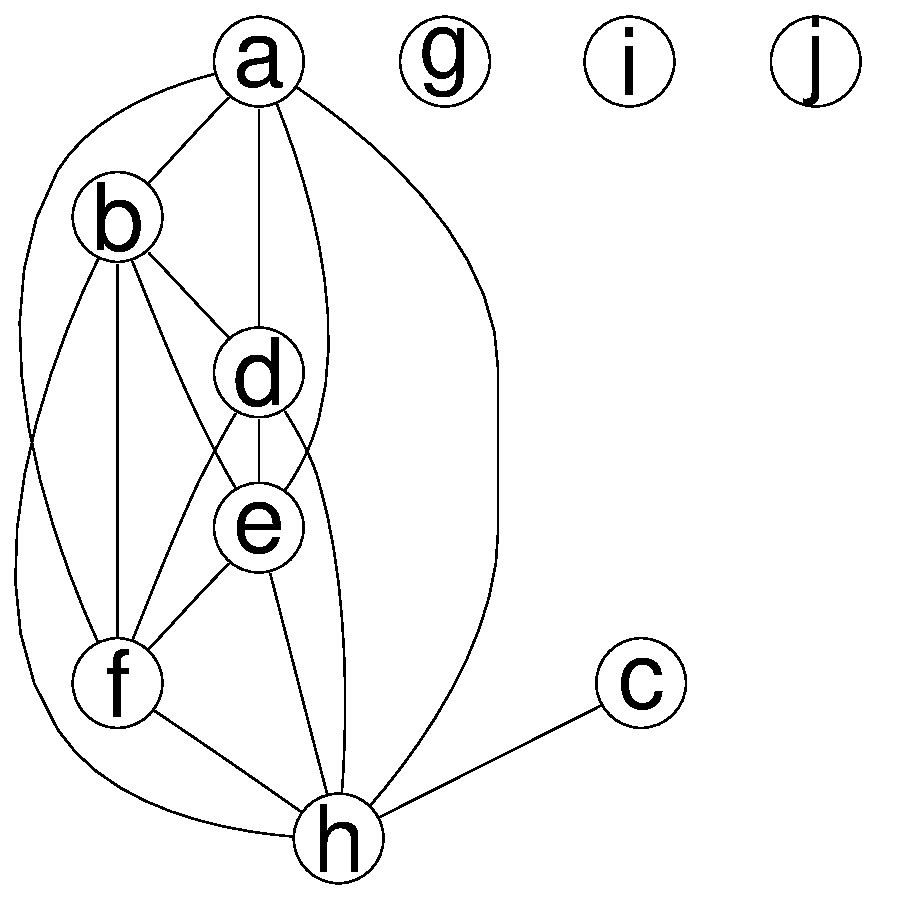
\includegraphics{newRgraphvizInterface-createGraph1}


%- - - - - - - - - - - - - - - - - - - - - - - - - - - - - - - - - - - 
\section{Default rendering parameters}
%- - - - - - - - - - - - - - - - - - - - - - - - - - - - - - - - - - -
There is a hierarchy to set rendering parameters for a graph. The
levels of this hierarchy are
\begin{enumerate}
  
\item{The session:} These are the defaults that will be used for a
  parameter if not set somewhere further down the hierarchy. You can
  change the session defaults at any time using the function
  \Rfunction{graph.par}.
  
\item{Rendering operation:} Defaults can be set for a single rendering
  operation, that is, for a single call to \Rfunction{renderGraph}
  using its \Robject{graph.pars} argument.
  
\item{Individual nodes or edges:} Parameters for individual nodes or
  edges in a graph object can be set using the
  \Rfunction{nodeRenderInfo} and \Rfunction{edgeRenderInfo} functions.
  
\end{enumerate}

Note that all parameters set in \Rfunction{renderGraph's}
\Robject{graph.pars} argument are transient, whereas setting
session-wide parameters will affect all subsequent rendering
operations. Setting parameters via the \Rfunction{nodeRenderInfo} and
\Rfunction{edgeRenderInfo} functions affects the individual graph
objects, and these changes will obviously be retained in all
subsequent layout or rendering operations of that particular graph.


%- - - - - - - - - - - - - - - - - - - - - - - - - - - - - - - - - - - 
\subsection{Default node parameters}
%- - - - - - - - - - - - - - - - - - - - - - - - - - - - - - - - - - -
We now use our example graph to further explore these options. Let's
start with the nodes: We want to fill all our nodes with a gray color
and use a red color for the node names. Since this should be applied
to all nodes, we set a global rendering parameter using
\Rfunction{graph.par}:
\begin{Schunk}
\begin{Sinput}
> graph.par(list(nodes=list(fill="lightgray", textCol="red")))
> renderGraph(g1)
\end{Sinput}
\end{Schunk}
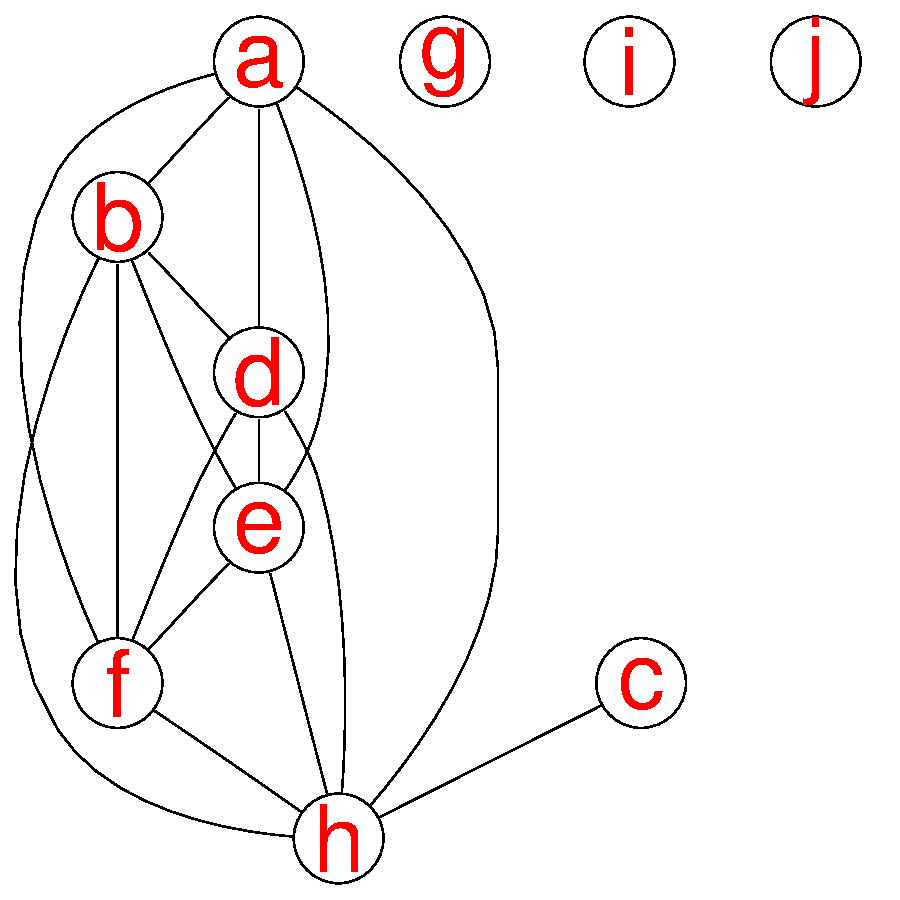
\includegraphics{newRgraphvizInterface-bgandfontcol}

Setting a session-wide parameter has side-effects for all subsequent
rendering operations, and we will soon see how to archive the same
setting using the \Rfunction{nodeRenderInfo} function. 

Note that \Rfunction{graph.par} takes as single argument a list of
rendering parameters. There are three different types of parameters
the user might want to set: nodewide parameters, edgewide parameters
and parameters that control features of the whole graph. Accordingly,
the parameters list passed to \Rfunction{graph.par} may contain the
list items \Robject{nodes}, \Robject{edges} and \Robject{graph}. Each
of these list items can again be a list of available plotting
parameters. In our example, the parameters are \Robject{fill} and
\Robject{textCol}. All currently available node parameters are:

\begin{itemize}
\item{col:} {the color of the line drawn as node border. Defaults to
  \Robject{black}.}
\item{lty:} {the type of the line drawn as node border. Defaults to
  \Robject{solid}. Valid values are the same as for the R's base
  graphic parameter \Robject{lty}.}
\item{lwd:} {the width of the line drawn as node border. Defaults to
  \Robject{1}.Note that the underlying low level plotting functions
  do not support vectorized \Robject{lwd} values. Instead, only the
  first item of the vector will be used.}
\item{fill:} {the color used to fill a node. Defaults to
  \Robject{transparent}.}
\item{textCol:}{the font color used for the node labels. Defaults to
  \Robject{black}.}
\item{fontsize:} {the font size for the node labels in
  points. Defaults to \Robject{14}. Note that the fontsize will be
  automatically adjusted to make sure that all labels fit their
  respective nodes. You may want to increase the node size by
  supplying the appropriate layout parameters to \textit{Graphviz} in
  order to allow for larger fontsizes.}
\item{cex:} {Expansion factor to further control the fontsize. As
  default, this parameter is not set, in which case the fontsize will
  be clipped to the node size. This mainly exists to for consistency
  with the base graphic parameters and to override the clipping of
  fontsize to nodesize.}
\item{shape:} {This is not really a graphical parameter. See Section
    \ref{layoutpars} for details.}

\end{itemize}

In the next code chunk we set the defaults for all remaining node parameters:
\begin{Schunk}
\begin{Sinput}
> graph.par(list(nodes=list(col="darkgreen", lty="dotted", lwd=2, fontsize=6)))
> renderGraph(g1)
\end{Sinput}
\end{Schunk}
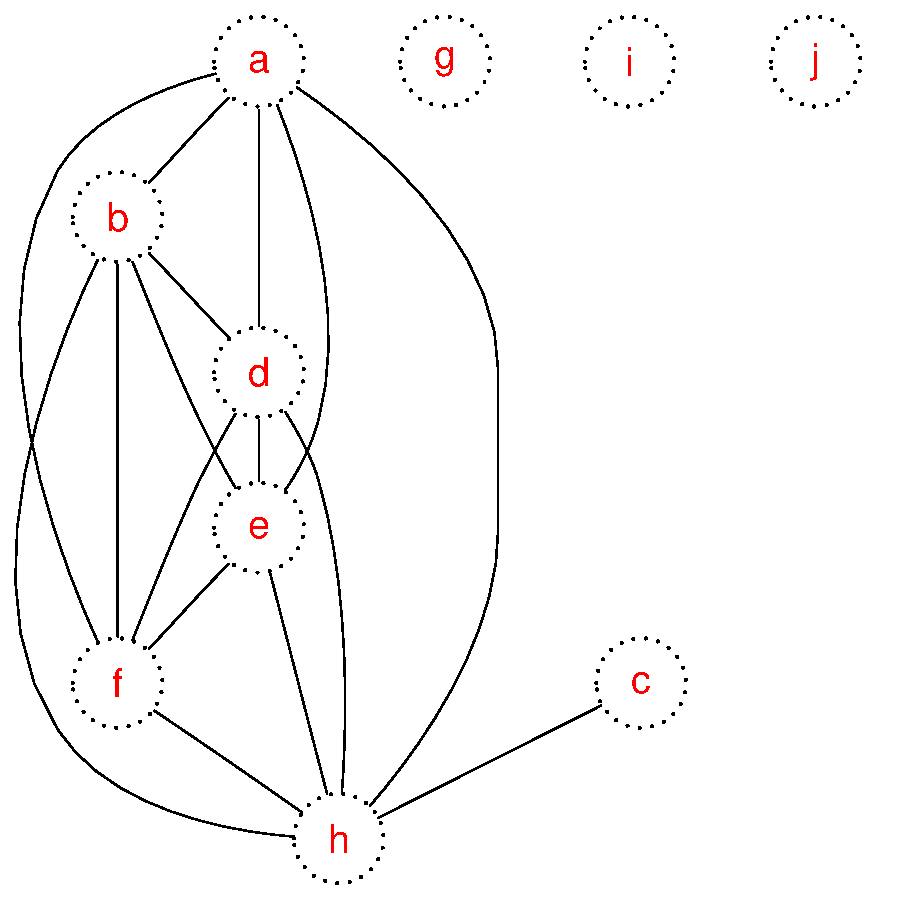
\includegraphics{newRgraphvizInterface-nodepardefs}

Similar to \R{}'s base \Rfunction{par} function, the original values
of a modified paramter are returned by \Rfunction{graph.par} and you
may want to assign them to an object in order to later revert your
changes.

A useful feature when plotting graphs is to control the shape of the
nodes. However, shapes have an impact on the ideal location of nodes
and, even more so, the edges between them. Hence, the layout algorithm
needs to be re-run whenever there are changes in node shapes. In
Section \ref{layoutpars} we will learn how to control node shapes and
also some features of the edges.

%- - - - - - - - - - - - - - - - - - - - - - - - - - - - - - - - - - - 
\subsection{Default edge parameters}
%- - - - - - - - - - - - - - - - - - - - - - - - - - - - - - - - - - -
Now, let's take a look at the parameters that control the appearence
of edges. They are:

\begin{itemize}
\item{col:} {the color of the edge line. Defaults to \Robject{black}.}
\item{lty:} {the type of the edge line. Defaults to
  \Robject{solid}. Valid values are the same as for the R's base
  graphic parameter \Robject{lty}.}
\item{lwd:} {the width of the edge line. Defaults to \Robject{1}.}
\item{textCol:}{the font color used for the edge labels. Defaults to
  \Robject{black}.}
\item{fontsize:} {the font size for the edge labels in points. Defaults
  to \Robject{14}.}
\item{cex:} {Expansion factor to further control the fontsize. This
  mainly exists to be consistent with the base graphic parameters.}
\item{arrowhead, arrowtail} {Again, not really a plotting
    parameter. Section \ref{layoutpars} provides details. }
\end{itemize}

First, we set some attributes that control the edge lines.
\begin{Schunk}
\begin{Sinput}
> graph.par(list(edges=list(col="lightblue", lty="dashed", lwd=3)))
> renderGraph(g1)
\end{Sinput}
\end{Schunk}
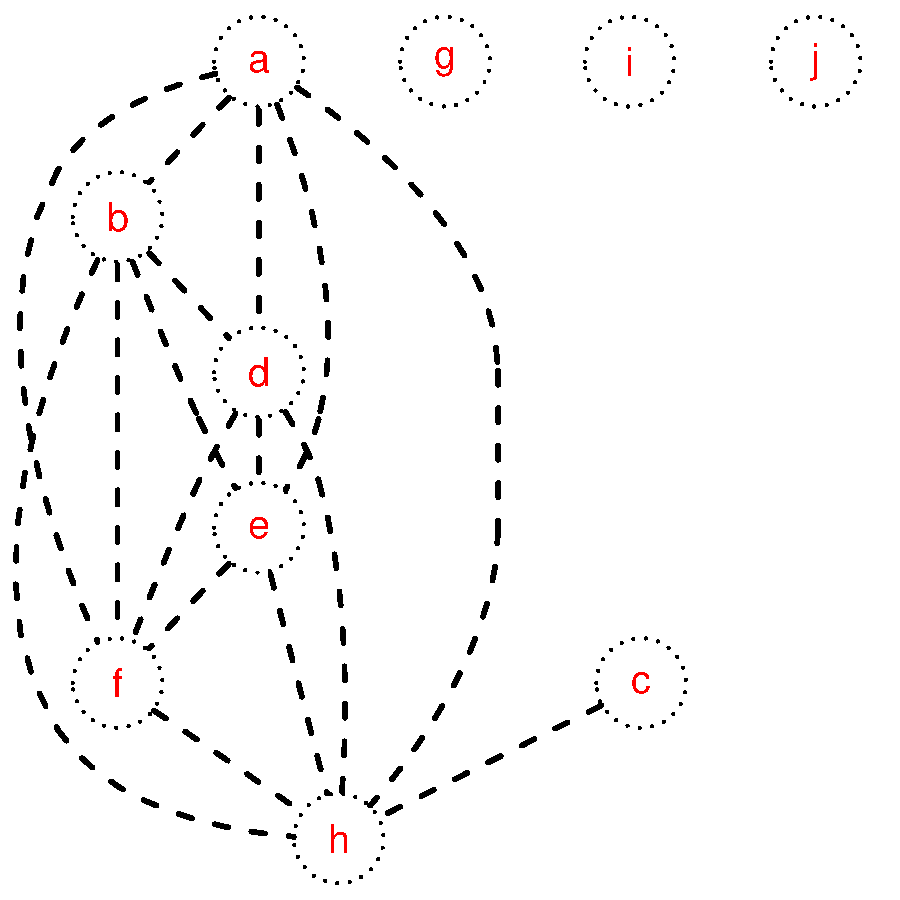
\includegraphics{newRgraphvizInterface-edgepardefs}

In order to show the effects of the edge label parameters, we first
have to add such labels. \Rfunction{layoutGraph} will pass them on to
\textit{Graphviz} when they are specified as \Robject{edgeAttrs}:
\begin{Schunk}
\begin{Sinput}
> labels <- edgeNames(g1)
> names(labels) <- labels
> g1 <- layoutGraph(g1, edgeAttrs=list(label=labels))
> renderGraph(g1)
\end{Sinput}
\end{Schunk}
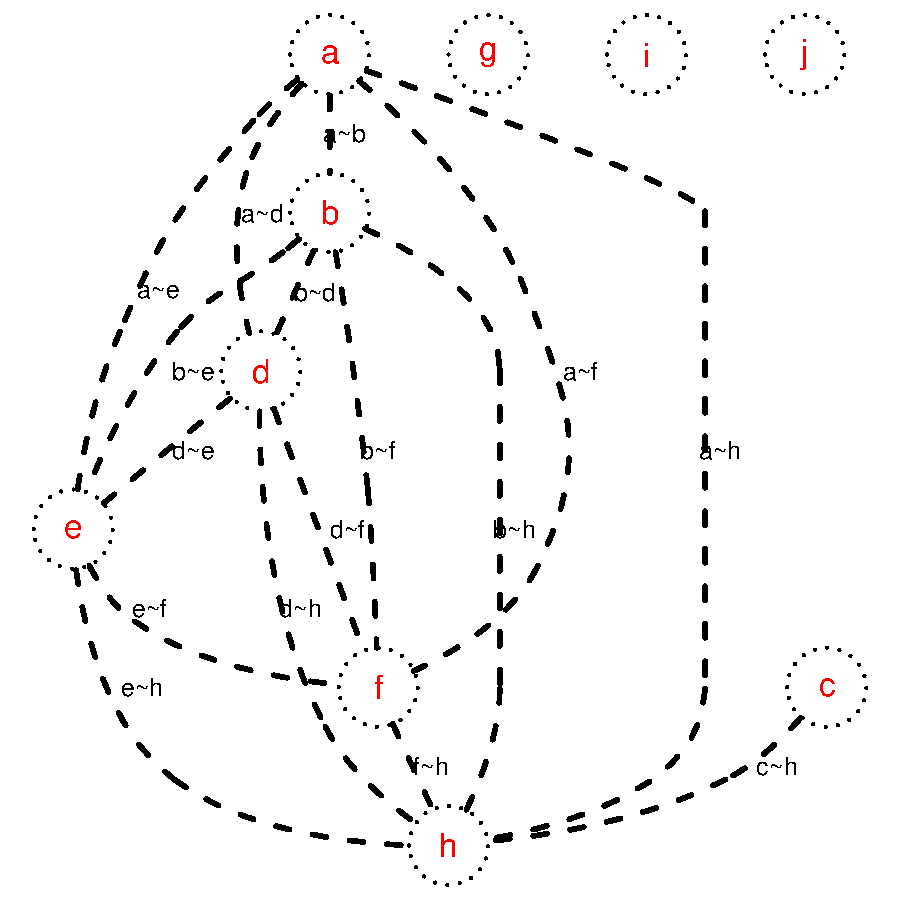
\includegraphics{newRgraphvizInterface-labels}

Now we can start tweaking them:
\begin{Schunk}
\begin{Sinput}
> graph.par(list(edges=list(fontsize=18, textCol="darkred")))
> renderGraph(g1)
\end{Sinput}
\end{Schunk}
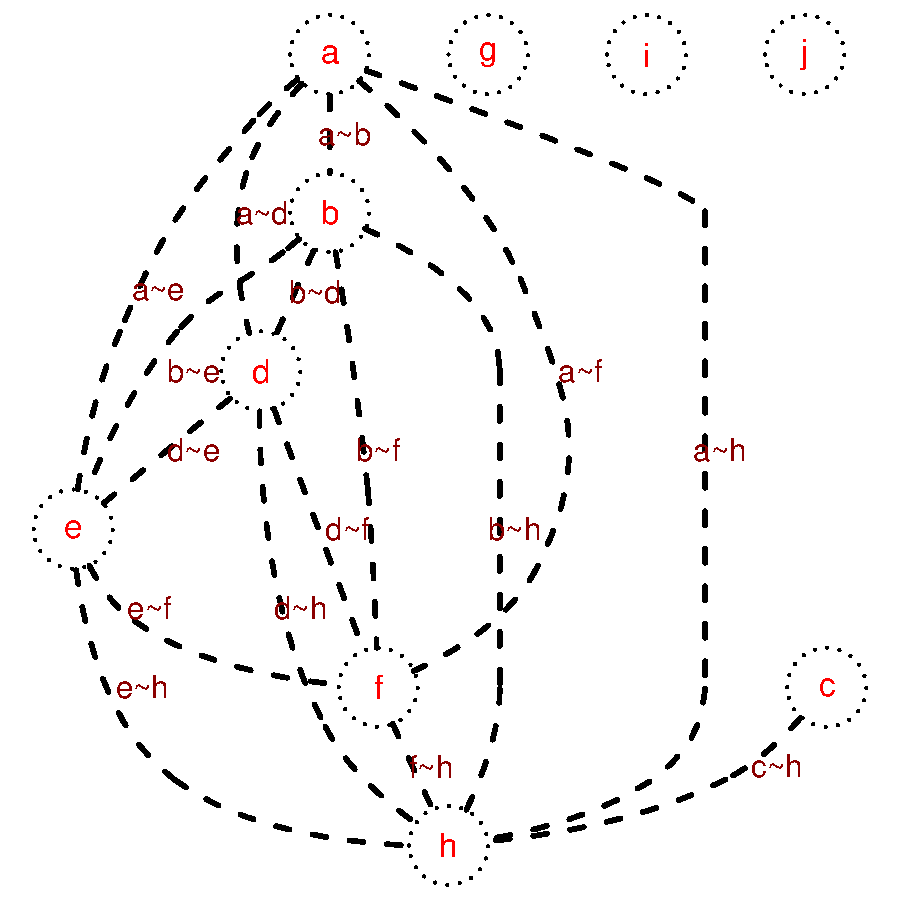
\includegraphics{newRgraphvizInterface-tweaklabesl}


%- - - - - - - - - - - - - - - - - - - - - - - - - - - - - - - - - - - 
\subsection{Default graphwide parameters}
%- - - - - - - - - - - - - - - - - - - - - - - - - - - - - - - - - - -
Some features of a graph are not really attributes of either nodes or
edges. They can be controlled through the graphwide rendering
parameters:

\begin{itemize}
\item{main:} {text that is plotted as the main title. Unless set
  explicitely, no title will be plotted.}
\item{sub:} {text that is plotted as subtitle at the bottom of the
  graph. Unless set explicitely, no subtitle will be plotted.}
\item{col.main:} {the font color used for the title. Defaults
  to \Robject{black}.}
\item{cex.main:} {Expansion factor for the fontsize used for the
  title. Defaults to \Robject{1.2}}
\item{col.sub:} {the font color used for the subtitle. Defaults
  to \Robject{black}.}
\item{cex.sub:} {Expansion factor for the fontsize used for the
  subtitle. Defaults to \Robject{1}}
\end{itemize}


Here, we add both a title and a subtitle to the plot.
\begin{Schunk}
\begin{Sinput}
> graph.par(list(graph=list(main="A main title...", 
+                sub="... and a subtitle", cex.main=1.8, 
+                cex.sub=1.4, col.sub="gray")))
> renderGraph(g1)
\end{Sinput}
\end{Schunk}
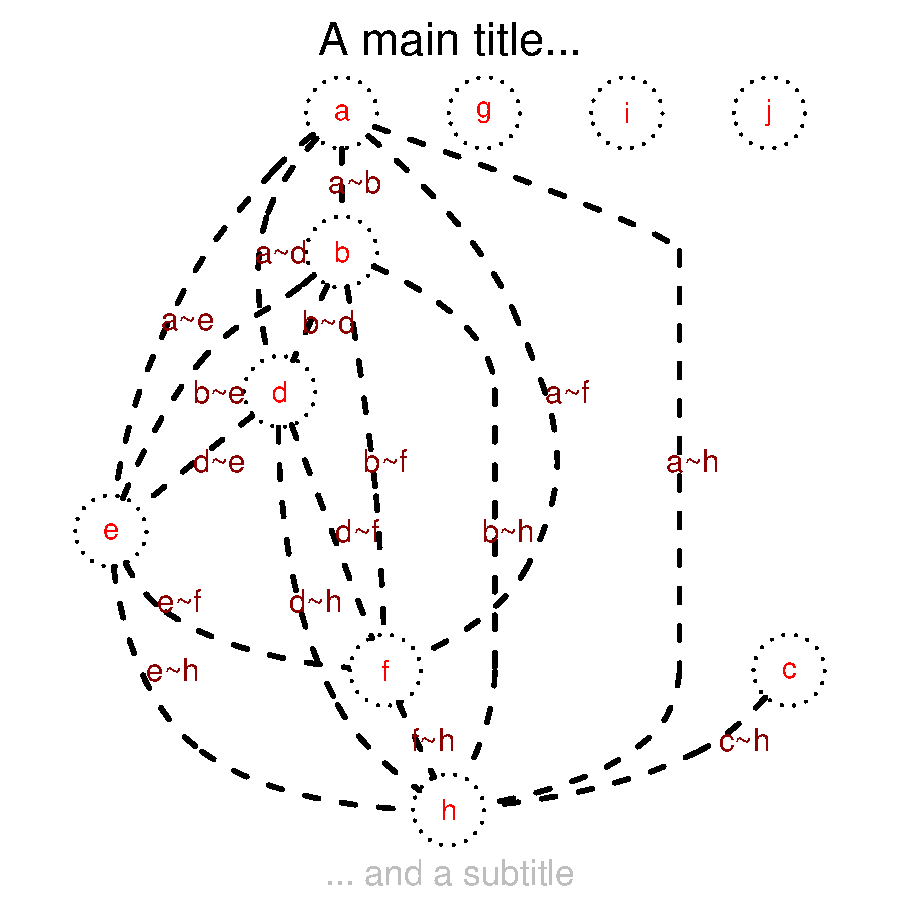
\includegraphics{newRgraphvizInterface-graphpardefs}

Of course we could set all graph-, node-, and edgewide parameters in
one single call to \Rfunction{graph.par}. Instead of defining global
settings with \Rfunction{graph.par} we could also provide a list with
the same structure to \Rfunction{renderGraph} through its
\Robject{graph.pars} argument. Those will only be applied in the
respective rendering operation, whereas options set using the function
\Rfunction{graph.par} are retained throughout the whole \R{} session.


%- - - - - - - - - - - - - - - - - - - - - - - - - - - - - - - - - - - 
\section{Parameters for individual nodes/edges} 
%- - - - - - - - - - - - - - - - - - - - - - - - - - - - - - - - - - -
In many cases we don't want to globally change certain parameters for
all nodes or edges, but rather do this selectively to highlight
individual nodes/edges or subsets thereof. To this end, parameters for
individual nodes and edges can be set using the
\Rfunction{nodeRenderInfo} and \Rfunction{edgeRenderInfo}
functions. Both \Rfunction{nodeRenderInfo} and
\Rfunction{edgeRenderInfo} are replacement functions that operate
directly on the \Rclass{graph} object. For completeness,
\Rfunction{graphRenderInfo} is the function that can be used to
control the graph-wide attributes (like captions and subtitles). When
you change a parameter in the \Rclass{graph} object this will be
carried on across all further rendering and layout operations. The
settings made by \Rfunction{edgeRenderInfo} and
\Rfunction{nodeRenderInfo} take precedence over all other default
settings.

The parameters to be set have to be given as named lists, where each
list item can contain named vectors for certain options. For example,
the following code sets the fill color of nodes \Robject{a} and
\Robject{b} to \Robject{yellow}.
\begin{Schunk}
\begin{Sinput}
> nodeRenderInfo(g1) <- list(fill=c(a="lightyellow", b="lightyellow"))
> renderGraph(g1) 
\end{Sinput}
\end{Schunk}
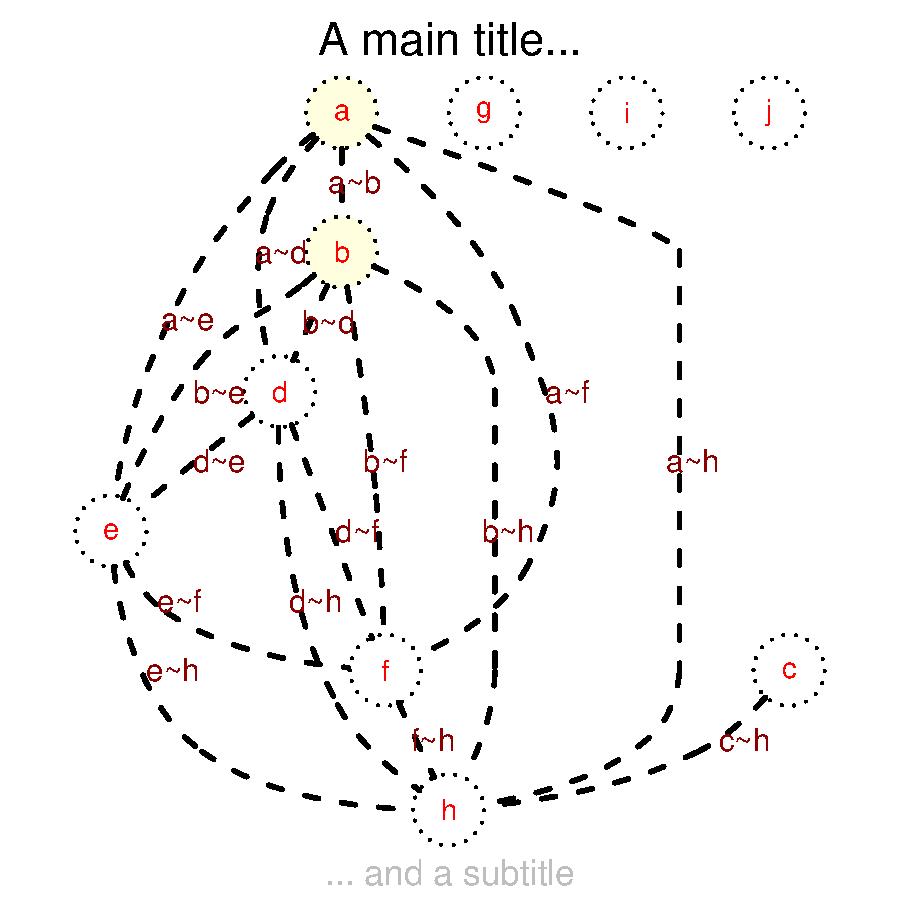
\includegraphics{newRgraphvizInterface-nodePars}

The names of the vectors have to match the node or edge names of the
graph. Node names are straightforward (the result of calling the
function \Rfunction{nodes} on a \Rclass{graph} object), however edge
names are made up of the names of the connected nodes separated by
\verb+~+, the tilde symbol.  An edge between nodes \verb+a+ and
\verb+b+ would be named \verb+a~b+. For a directed graph \verb+a~b+ is
the edge fom \verb+a+ to \verb+b+, and \verb+b~a+ is the edge from
\verb+b+ to \verb+a+. For undirected graphs the two are
equivalent. \Rfunction{edgeNames} returns the names of all edges in a
graph. The following code changes the line type of the edges between
nodes \verb+b+ and \verb+f+ and nodes \verb+b+ and \verb+h+ to
\Robject{solid} and their line color to \Robject{orange}.

\begin{Schunk}
\begin{Sinput}
> edgeRenderInfo(g1) <- list(lty=c("b~f"="solid", "b~h"="solid"),
+                           col=c("b~f"="orange", "b~h"="orange"))
> renderGraph(g1)
\end{Sinput}
\end{Schunk}
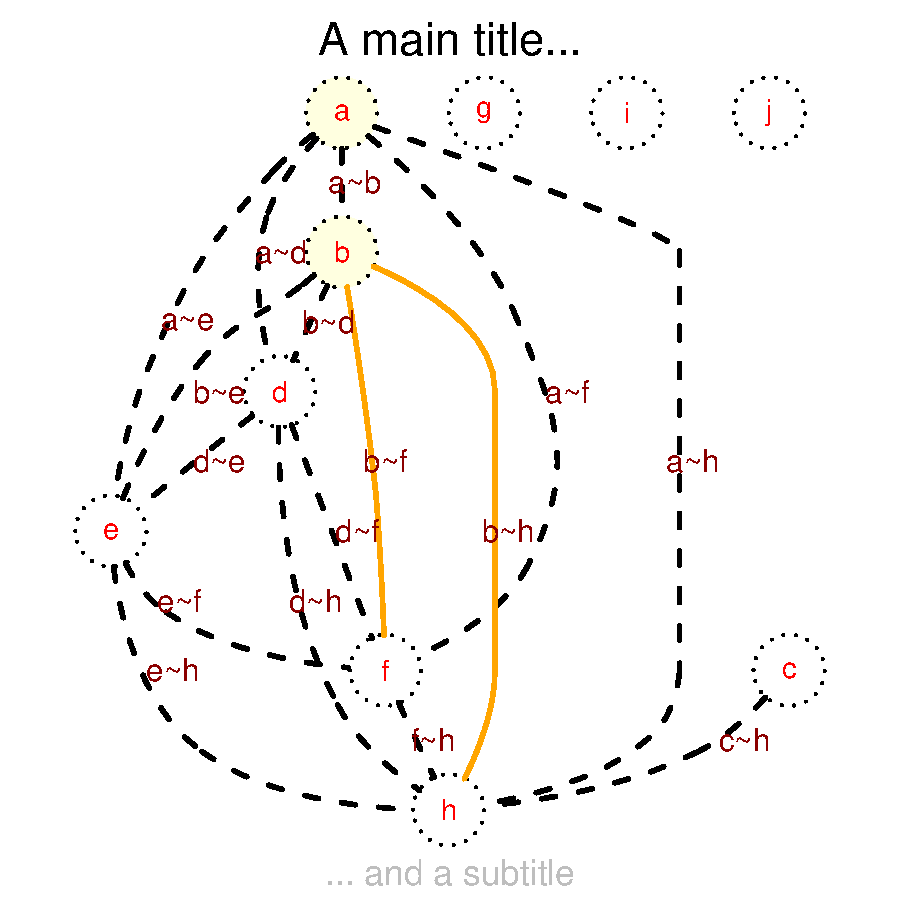
\includegraphics{newRgraphvizInterface-edgePars}

Changes in the rendering of specific nodes or edges is often motivated
by certain classes or features they represent and we don't want to set
this manually but rather use a programmatic approach:
\begin{Schunk}
\begin{Sinput}
> baseNodes <- letters[1:4]
> fill <- rep("lightblue", length(baseNodes))
> names(fill) <- baseNodes
> nodeRenderInfo(g1) <- list(fill=fill)
> renderGraph(g1)
\end{Sinput}
\end{Schunk}
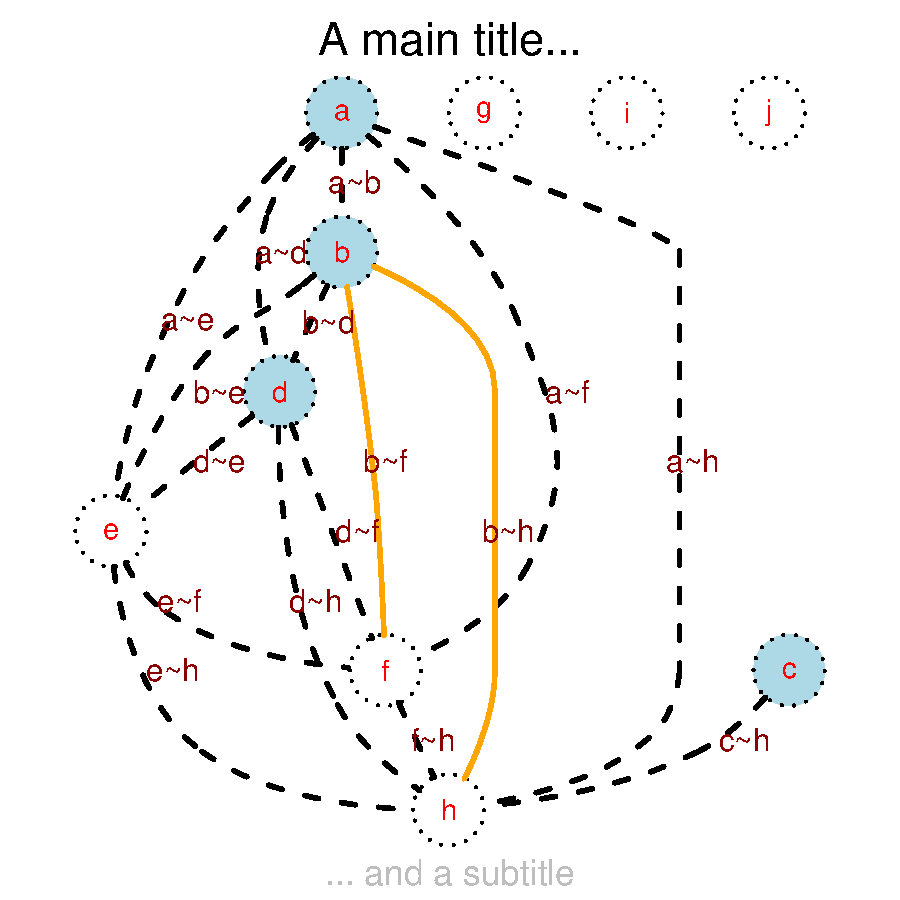
\includegraphics{newRgraphvizInterface-programParms}

Both \Rfunction{nodeRenderInfo} and
\Rfunction{edgeRenderInfo} also allow to set parameters for all edges
or nodes of the graph at once. The syntax is simple: instead of a
named vector one can pass a scalar for a given parameter. This value
will then be assigned to all available nodes or edges.

\begin{Schunk}
\begin{Sinput}
> nodeRenderInfo(g1) <- list(lty=1)
> edgeRenderInfo(g1) <- list(lty=1, lwd=2, col="gray")
> renderGraph(g1)
\end{Sinput}
\end{Schunk}
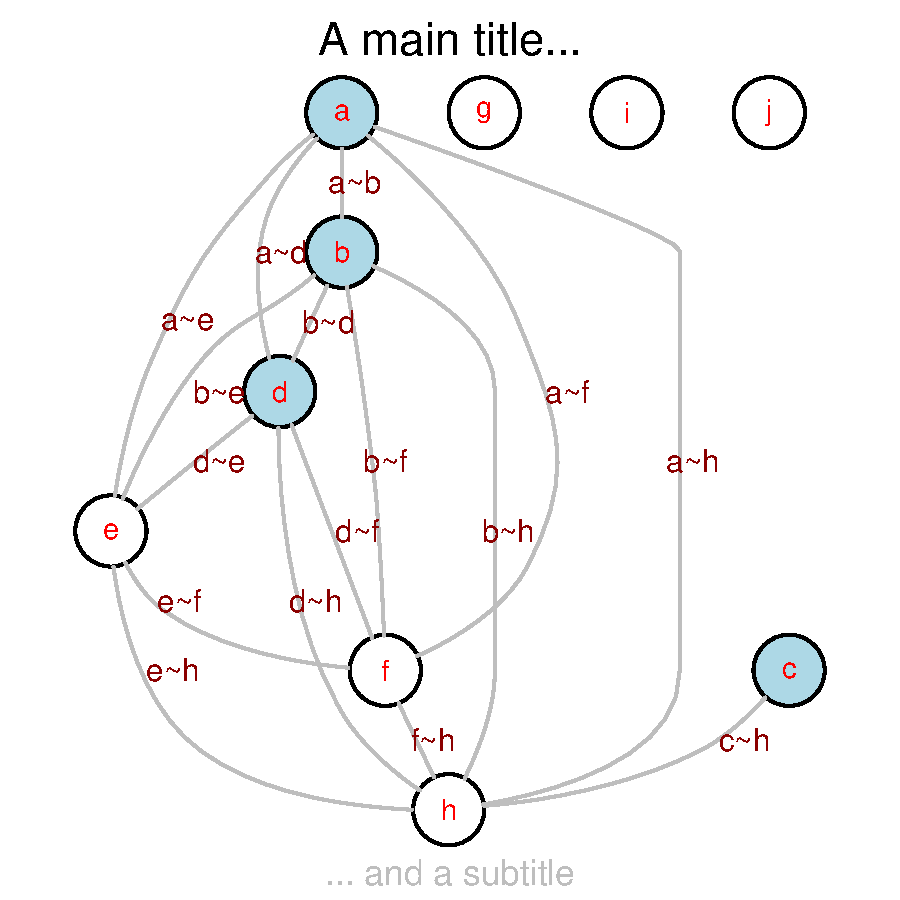
\includegraphics{newRgraphvizInterface-setallatonce}

The easiest way to set an attribute back to its default (the session
default if it has been set) is to pass in a \Robject{NULL} list item
via the respective setter function.

\begin{Schunk}
\begin{Sinput}
> nodeRenderInfo(g1) <- list(fill=list(b=NULL, d=NULL))
> renderGraph(g1)
\end{Sinput}
\end{Schunk}
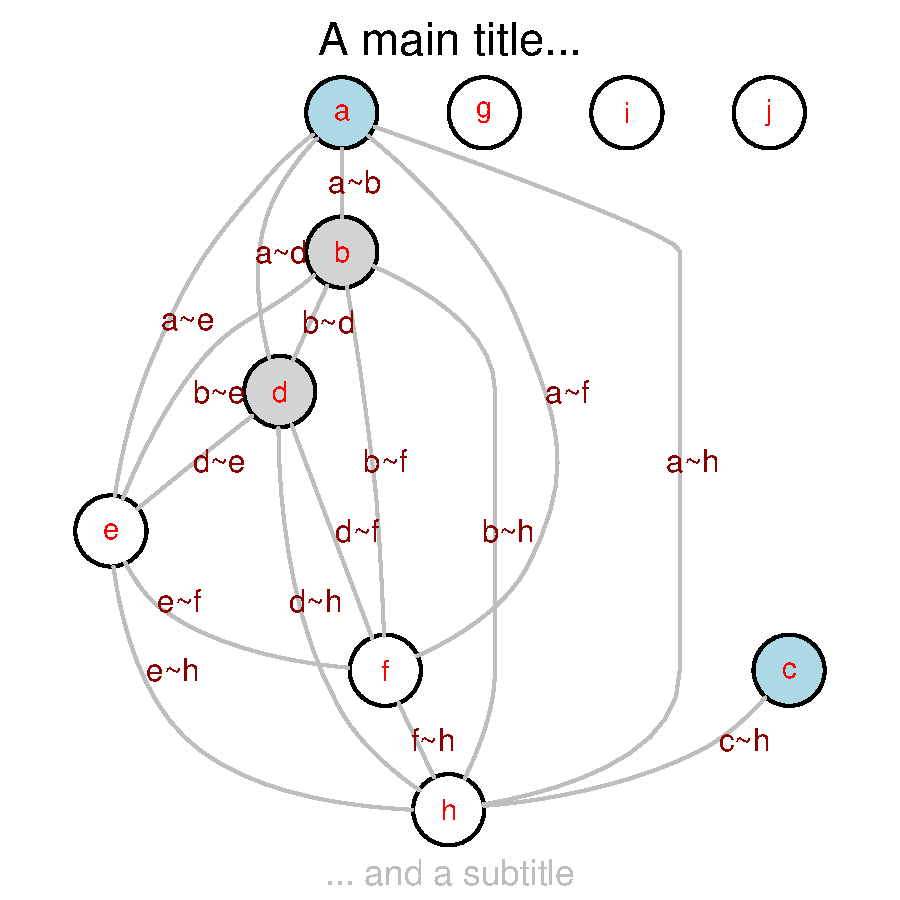
\includegraphics{newRgraphvizInterface-reset}


\section{Graphical parameters that affect the layout}\label{layoutpars}
As mentioned before, some graphical parameters are somewhat on the
border between graph layout and graph rendering. The shape of the node
for example does not drastically affect it's location, however the
layout of the edges pointing to and from this node might slightly
change. Since manipulating these attributes is a frequent operation in
graph plotting, we decided to make them available through the
rendering interface.

\subsection{Node shapes}
Node shapes can be set using the \Robject{shape} parameter. Currently,
the rendering function supports the following shape types:

\begin{itemize}
\item{circle} {this is the default value. Circular nodes are not
    affected by changes in width or height, the algorithm will
    always use a quadratic bounding box}
\item{ellipse} {this shape allows for differences in width and
    height. Elliptical nodes often fit node labels better without
    wasting too much real estate. }
\item{box, rectangle} {A rectangular node.}
\item{triangle}  {this  is  currently  only partly  supported  due  to
    restrictions in the Graphviz  interface. Edges locations might not
    be optimal when triangular nodes are used.}
\item{plaintext} {no node shape at all, only the node labels are
    plotted.}
\end{itemize}

Lets change all nodes shapes to ellipses first and then try out some
of the remaining shapes on single nodes. Because of their impact on
the overall layout, we have to run \Rfunction{layoutGraph} again in
order for these modifications to work.
\begin{Schunk}
\begin{Sinput}
> nodeRenderInfo(g1) <- list(shape="ellipse")
> nodeRenderInfo(g1) <- list(shape=c(g="box", i="triangle", 
+                                    j="circle", c="plaintext"))
> g1 <- layoutGraph(g1)
> renderGraph(g1)
\end{Sinput}
\end{Schunk}
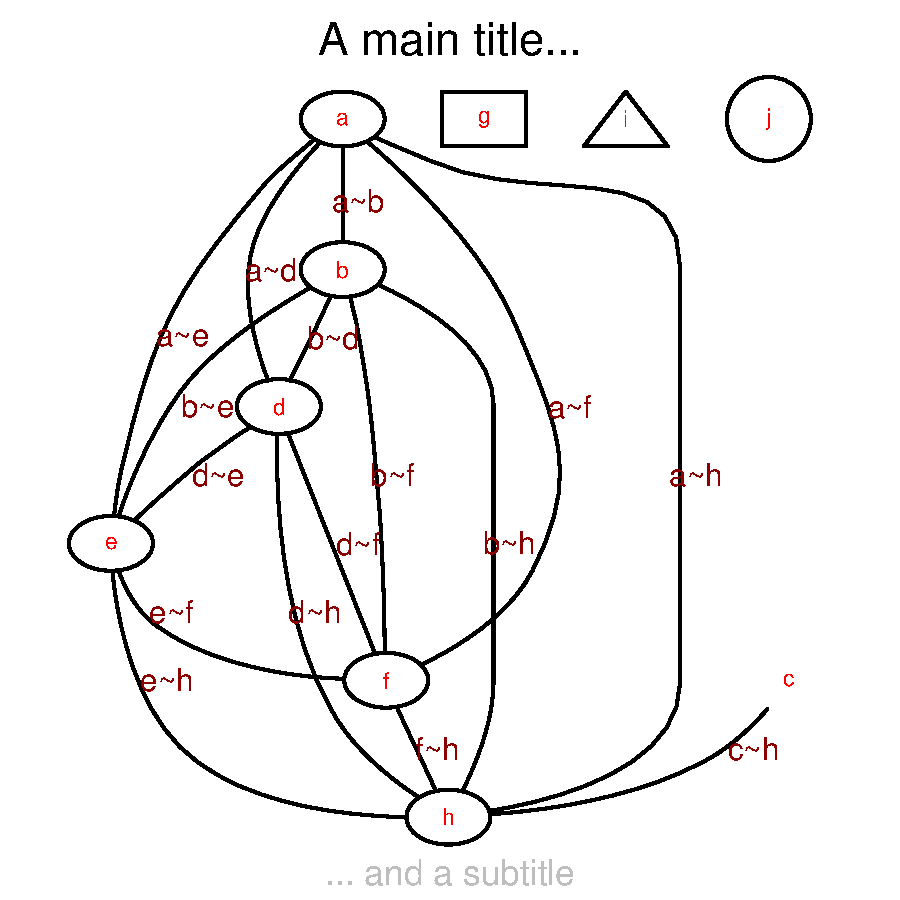
\includegraphics{newRgraphvizInterface-nshape}

To provide even more flexibility, the values of the \Robject{shape}
attributes can also be user-defined functions. \Rfunction{renderGraph}
will call these functions internally, passing on a number of
parameters. The most important parameter is a two-by-two matrix giving
the bounding box of the respective node. This information should be
used in the self-defined node plotting function to control the node
location and also its size. No clipping ever occurs to this bounding
box, and if the user decides to extend the node size beyond these
limits, overplotting with other nodes or edges is very likely. The
additional parameters that are passsed on to the function are:
\Robject{labelX}, \Robject{labelY}, \Robject{fill}, \Robject{col},
\Robject{lwd}, \Robject{lty}, \Robject{textCol}, \Robject{style},
\Robject{label} and \Robject{fontsize}. Consult the help pages of the
\Rfunction{layoutGraph} and \Rfunction{renderGraph} functions for
details.

As an example we will use a function that creates random thermometer
plots as node glyphs in the following code chunk. Note that we make
use of the \Robject{...} argument to catch all of the passed
parameters that we don't really need. We also remove the edge labels
from the graph to tidy it up a little.
\begin{Schunk}
\begin{Sinput}
> edgeRenderInfo(g1) <- list(label=NULL)
> myNode <- function(x, col, fill, ...)
+ symbols(x=mean(x[,1]), y=mean(x[,2]), thermometers=cbind(.5, 1,
+ runif(1)), inches=0.5,
+ fg=col, bg=fill, add=TRUE)
> nodeRenderInfo(g1) <- list(shape=list(d=myNode, f=myNode), 
+                            fill=c(d="white", f="white"),
+                            col=c(d="black", f="black"))
> g1 <- layoutGraph(g1)
> renderGraph(g1)
\end{Sinput}
\end{Schunk}
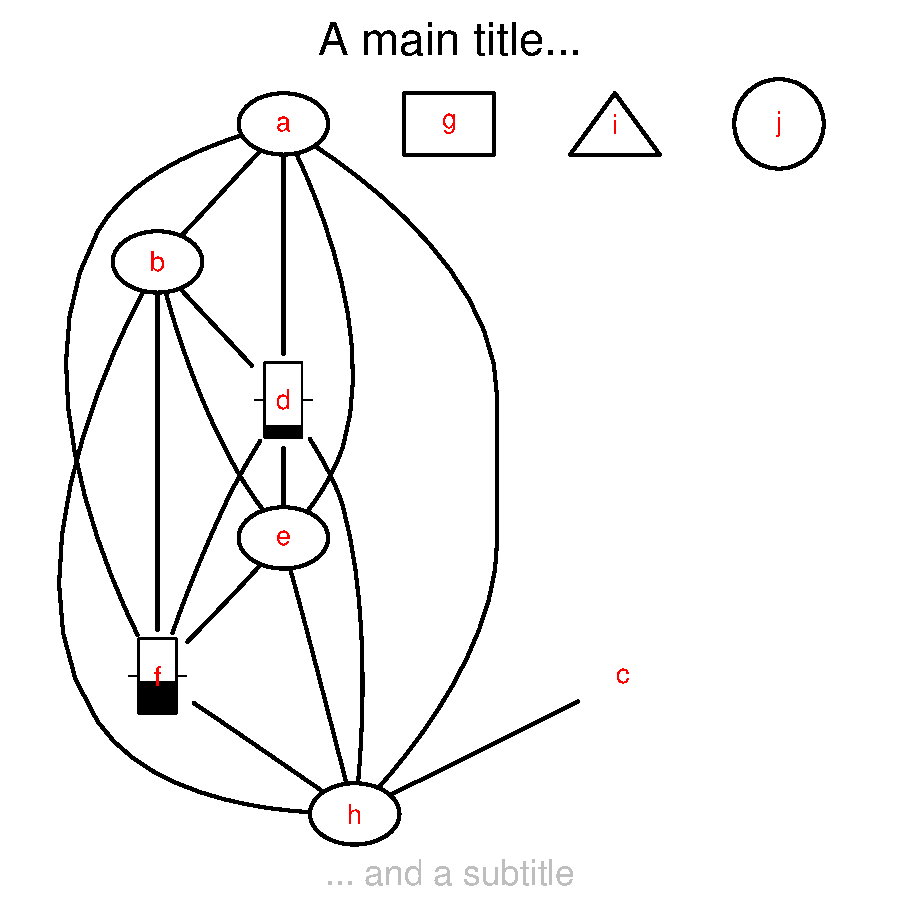
\includegraphics{newRgraphvizInterface-userDefinedNode}

\subsection{Edge arrowheads and arrowtails}

Similar to the control of node shapes, \Rfunction{renderGraph}
supports different types of shapes for the tips of the edges. In
undirected graphs this feature is not really supported because edges
are merely connecting nodes, they don't convey any information about
direction. We can change the mode of our sample graph to
\Robject{directed} to further explore this feature.
\begin{Schunk}
\begin{Sinput}
> edgemode(g1) <- "directed"
\end{Sinput}
\end{Schunk}

The valid values for both arrowheads and arrowtails of the edges are
\Robject{open}, \Robject{normal}, \Robject{dot}, \Robject{odot},
\Robject{box}, \Robject{obox}, \Robject{tee}, \Robject{diamond},
\Robject{odiamond} and \Robject{none}. The little helper function
\Rfunction{edgeNames} can be used to list all available edge names.
\begin{Schunk}
\begin{Sinput}
> edgeRenderInfo(g1) <- list(arrowhead=c("e~h"="dot", "c~h"="odot",
+                                        "a~h"="diamond", "b~f"="box",
+                                        "a~b"="box", "f~h"="odiamond"),
+                            arrowtail="tee")
> g1 <- layoutGraph(g1)
> renderGraph(g1)
\end{Sinput}
\end{Schunk}
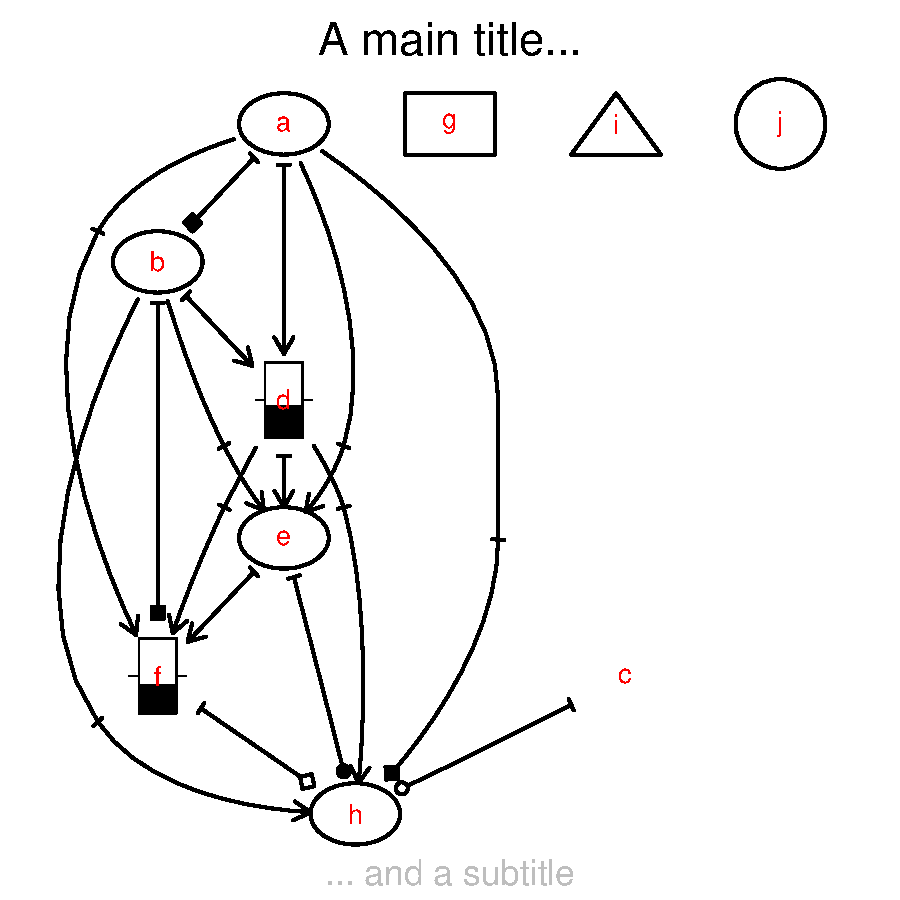
\includegraphics{newRgraphvizInterface-arrowheads}

There is also the option to pass a user-defined function as
\Robject{arrowhead} or \Robject{arrowtail} parameter to gain even more
control. Similar to node shapes, the function has to be able to deal
with several parameters: The first parameter gives the center of the
location of the arrowhead or tail. The additional parameters
\Robject{col}, \Robject{lwd} and \Robject{lty} are color and line
styles defined for the edges.
\begin{Schunk}
\begin{Sinput}
> myArrows <- function(x, ...)
+ {
+ for(i in 1:3)
+ points(x,cex=i, ...)
+ }
> edgeRenderInfo(g1) <- list(arrowtail=c("c~h"=myArrows))
> g1 <- layoutGraph(g1)
> renderGraph(g1)
\end{Sinput}
\end{Schunk}
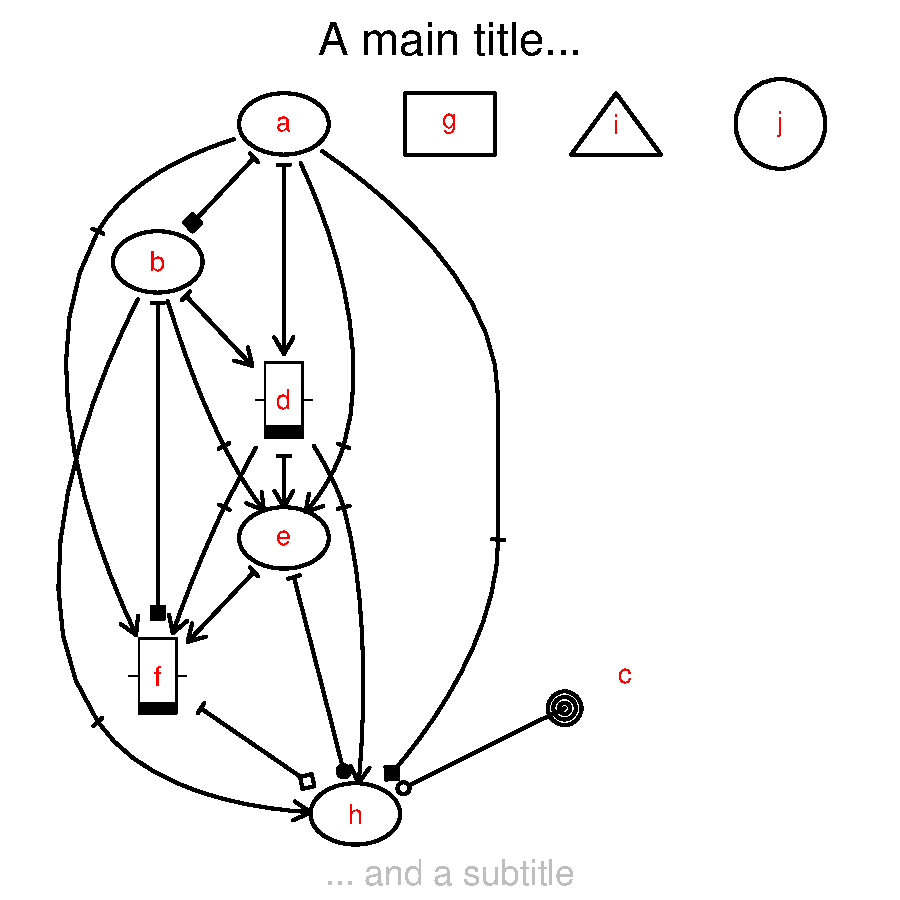
\includegraphics{newRgraphvizInterface-userDefinedEdge}



\section{Sessioninfo}

This document was produced using
\begin{Schunk}
\begin{Soutput}
R version 3.0.2 (2013-09-25)
Platform: i386-w64-mingw32/i386 (32-bit)

locale:
[1] LC_COLLATE=English_United States.1252 
[2] LC_CTYPE=English_United States.1252   
[3] LC_MONETARY=English_United States.1252
[4] LC_NUMERIC=C                          
[5] LC_TIME=English_United States.1252    

attached base packages:
[1] grid      stats     graphics  grDevices utils     datasets  methods  
[8] base     

other attached packages:
[1] Rgraphviz_2.6.0 graph_1.40.0   

loaded via a namespace (and not attached):
[1] BiocGenerics_0.8.0 parallel_3.0.2     stats4_3.0.2       tools_3.0.2       
\end{Soutput}
\end{Schunk}
together with version list(c(2, 28, 0)) of graphviz.


\end{document}
